\subsection*{1.1}
  % Implement  the  common-source  MOS  amplifier  shown  below.  The  transistor  model
  % should be modified to look as follows:
  % Cgs  2 3 20E-12 
  % Cgd 1 2 10E-12 
  % M1 1 2 3 3 MOST1 W=500u L=2u
  % .MODEL MOST1 NMOS(Level=3 Kp=20u W=500u L=2u Rs=20m Vto=2 Rd=1.186)
    \begin{figure}[h!]
        \centering
        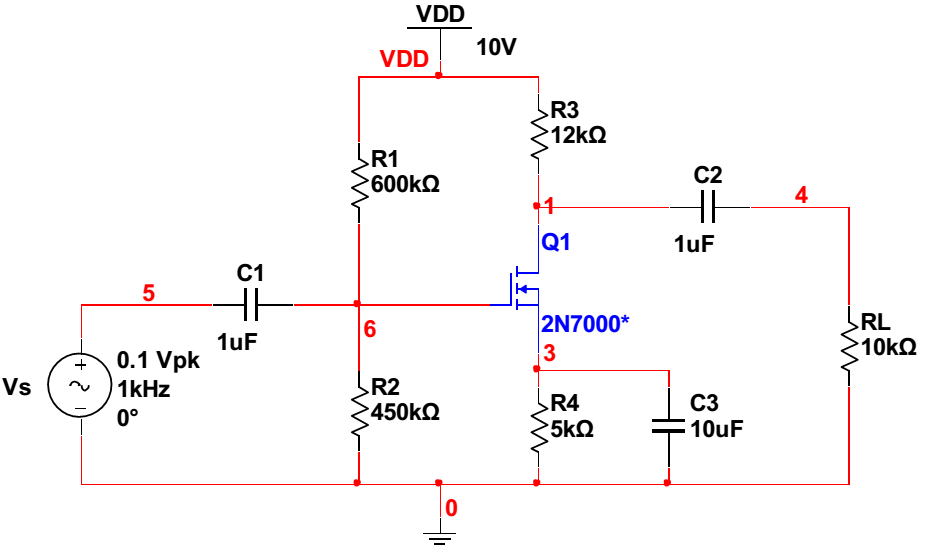
\includegraphics[width=6cm]{fig1-1.png}
        \captionof{figure}{The CS MOS amplifier to be implemented in Task 1.1}
    \end{figure} 
    

\subsection*{1.2}
  % Using  the  above  parameters  (here:  kn =  20  µA/V2,  W/L =  250,  VT =  2  V,  Cgs =  20  pF,
  % Cgd = 10 pF) perform the theoretical analysis of the circuit to find the voltage gain, input
  % resistance, output resistance, as well as to estimate the lower and upper 3dB frequencies.

\subsection*{1.3}
  % Determine the values of the same parameters by simulation. Note that in order to obtain
  % some  of  the  parameters  certain  changes  in  the  circuit  diagram  and/or  introducing  some
  % auxiliary elements may be necessary. 

\subsection*{1.4}
  % Compare the parameters obtained by simulation with those obtained from the theory and
  % comment upon possible differences.
  